%  !TeX  root  =  user_guide.tex
% % \section{Print Composer}\label{label_printcomposer}
\chapter{Composeur de carte}\label{label_printcomposer}

% when the revision of a section has been finalized, 
% comment out the following line:
% \updatedisclaimer

%The print composer provides growing layout and printing
%capabilities. It allows you to add elements such as the QGIS map canvas, 
%legend, scalebar, images, and text labels. You can size, group 
%align and position each element and adjust the properties to create your
%layout. The layout can be printed or exported to image formats, Postscript,
%PDF or to SVG \footnote{Export to SVG supported, but it is not working
%properly with some recent QT4 versions. You should try and
%check individual on your system} and you can save the layout as template and
%load it again in another session. See a list of tools in
%table~\ref{tab:printcomposer_tools}:
Le composeur de carte fournit des fonctionnalités croissantes de mise en page et d'impression. Il vous permet d'ajouter des éléments tels qu'un cadre de carte, une légende, une échelle graphique, des images, des flèches et des étiquettes. Vous pouvez modifier la taille, grouper, aligner et positionner chaque élément et ajuster leurs propriétés pour créer votre mise en page. Le résultat peut être imprimé ou exporté dans plusieurs formats d'images, mais aussi en Postscript, PDF et SVG.\footnote{L'export en SVG est géré, mais il ne fonctionne pas correctement avec certaines versions de QT4. Vous devriez essayer et vérifier individuellement sur votre système} Voici une liste des outils (tableau~\ref{tab:printcomposer_tools}) :

\begin{table}[p]\index{Composeur de carte!outils}
\centering\small
\renewcommand{\arraystretch}{2}
 \begin{tabular}{|m{1cm}|m{5.4cm}|m{1cm}|m{5.4cm}|}
 \hline \textbf{Icône} & \textbf{Objectif} & \textbf{Icône} &
 \textbf{Objectif} \\
\hline 
\includegraphics[width=0.7cm]{mActionFolder} & Charger depuis un modèle &
 
\includegraphics[width=0.7cm]{mActionFileSaveAs} & Enregistrer en tant que modèle \\
\hline 
\includegraphics[width=0.7cm]{mActionExportMapServer}  & Exporter dans un format d'image & 
 
\includegraphics[width=0.7cm]{mActionSaveAsPDF} & Exporter en PDF \\
\hline 
\includegraphics[width=0.7cm]{mActionSaveAsSVG} & Exporter la composition en SVG& \multicolumn{2}{c|}{}\\
\hline 
\includegraphics[width=0.7cm]{mActionFilePrint} & Imprimer ou exporter en Postscript &
 
\includegraphics[width=0.7cm]{mActionZoomFullExtent} & Zoom à l'étendue maximale\\
\hline 
\includegraphics[width=0.7cm]{mActionZoomIn} & Zoom + &
 
\includegraphics[width=0.7cm]{mActionZoomOut} & Zoom - \\
\hline 
\includegraphics[width=0.7cm]{mActionDraw} & Rafraichie la vue &
 
\includegraphics[width=0.7cm]{mActionAddMap} & Ajouter une nouvelle carte à partir du cadre de carte de QGIS \\
\hline 
\includegraphics[width=0.7cm]{mActionSaveMapAsImage} & Ajouter une image au composeur de carte &
 
\includegraphics[width=0.7cm]{mActionLabel} & Ajoute des étiquettes à la composition de carte \\
\hline 
\includegraphics[width=0.7cm]{mActionAddLegend} & Ajoute une nouvelle légende à la composition de carte &
 
\includegraphics[width=0.7cm]{mActionScaleBar} & Ajoute une barre d'échelle graphique à la composition de carte\\
\hline 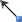
\includegraphics[width=0.7cm]{mActionAddArrow} & Ajoute une flèche à la composition & 
 
\includegraphics[width=0.7cm]{mActionOpenTable} & Add attribute table to print composition \\
\hline 
\includegraphics[width=0.7cm]{mActionSelectPan} & Sélectionne/déplace les objets dans la composition de carte &
 
\includegraphics[width=0.7cm]{mActionMoveItemContent} & Déplace le contenu dans un objet \\
\hline 
\includegraphics[width=0.7cm]{mActionGroupItems} & Groupe les objets de la composition de carte & 
 
\includegraphics[width=0.7cm]{mActionUngroupItems} & Désolidaise les objets de la composition de carte \\
\hline 
\includegraphics[width=0.7cm]{mActionRaiseItems} & Passe les objets par dessus dans la composition de carte &
 
\includegraphics[width=0.7cm]{mActionLowerItems} & Passe les objets par dessous dans la composition de carte \\
\hline 
\includegraphics[width=0.7cm]{mActionMoveItemsToTop} & Déplace les objets sélectionnés tout en haut & 
 
\includegraphics[width=0.7cm]{mActionMoveItemsToBottom} & Déplace les objets sélectionnés tout en bas \\
 \hline 
\includegraphics[width=0.7cm]{mActionAlignLeft} & Aligner les objets sélectionnés à gauche &
 
\includegraphics[width=0.7cm]{mActionAlignRight} & Aligner les objets sélectionnés à droite \\
 \hline 
\includegraphics[width=0.7cm]{mActionAlignHCenter} & Aligner les objets sélectionnés au centre &
 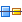
\includegraphics[width=0.7cm]{mActionAlignVCenter} & Aligner les objets sélectionnés au centre vertical \\
 \hline 
\includegraphics[width=0.7cm]{mActionAlignTop} & Aligner les objets sélectionnés vers le haut &
 
\includegraphics[width=0.7cm]{mActionAlignBottom} & Aligner les objets sélectionnés  vers le bas \\
\hline
\end{tabular}
\caption{Outils du Composeur de carte}\label{tab:printcomposer_tools}
\end{table}

%All Print Composer tools are availabe in menus and as icons in a toolbar. The
%toolbar can be switched off and on using the right mouse button holding the
%mouse over the toolbar.

Tous les outils de composition de carte pour l'impression sont disponibles dans les menus et la barre d'outils, cette barre peut être affichée ou masquée en faisant un clic droit au-dessus d'elle.

% \section{Using Print Composer}\label{label_useprintcomposer} 
\section{Utiliser le Composeur d'Impression}\label{label_useprintcomposer} 

% Before you start to work with the print composer, you need to load some 
% raster and vector layers in the QGIS map canvas and adapt their properties 
% to suite your own convinience. After everything is rendered and symbolized to 
% your liking you click the \toolbtntwo{mActionFilePrint}{Print Composer} icon.
Avant de démarrer le travail avec le composeur de carte, vous devez charger certaines couches raster et vecteurs dans la fenêtre de carte de QGIS et 
adapter leurs propriétés pour qu'elles vous conviennent. Après que tout soit rendu et symbolisé comme vous le souhaitez, cliquez sur l'icône \toolbtntwo{mActionFilePrint}{Nouveau composeur d'impression} ou le menu \mainmenuopt{Fichier} > \dropmenuopttwo{mActionNewComposer}{Nouveau composeur d'impression}.

%\begin{figure}[ht]
%   \begin{center}
%   \caption{Print Composer \nixcaption}\label{fig:print_composer_blank}\smallskip
%   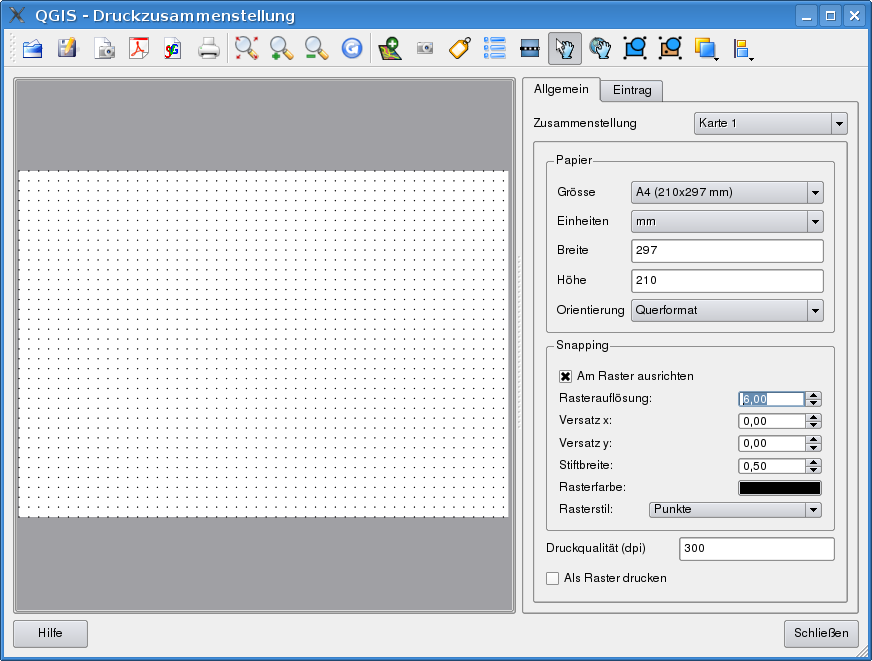
\includegraphics[clip=true, width=\textwidth]{print_composer_blank}
%\end{center}  
%\end{figure}

\begin{figure}[ht]
   \begin{center}
   \caption{Composeur de carte\nixcaption}\label{fig:print_composer_blank}\smallskip
   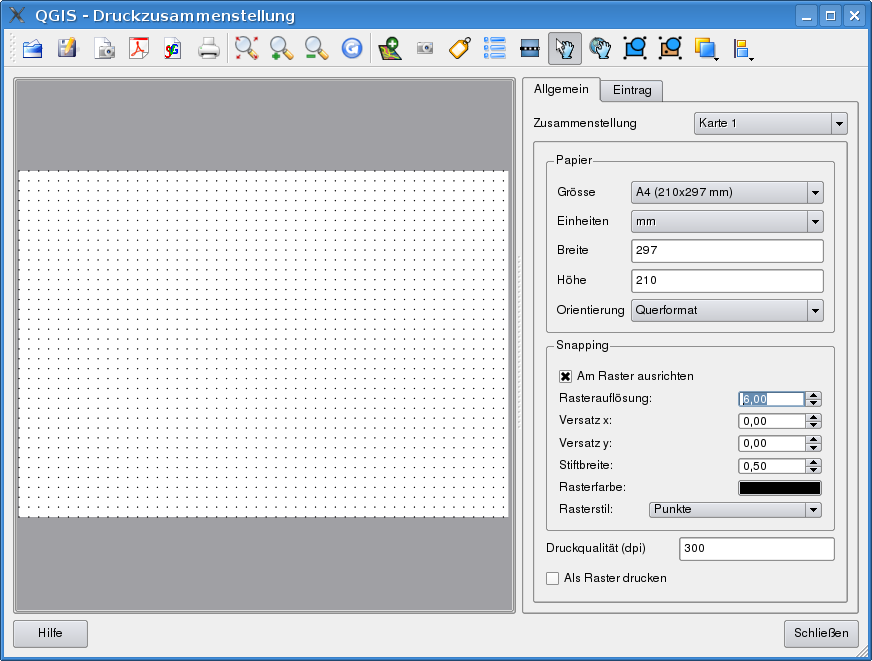
\includegraphics[clip=true, width=10cm]{print_composer_blank}
\end{center}
\end{figure}

% Opening the print composer provides you with a blank canvas to which you can 
% add the current QGIS map canvas, legend, scalebar, images and text. Figure
% \ref{fig:print_composer_blank} shows the initial view of the print composer 
% before any elements are added. The print composer provides two tabs:
Ouvrir le composeur de carte vous affiche un cadre vide auquel vous pouvez ajouter un cadre de la carte actuelle de QGIS, une légende, une échelle
graphique, des images et du texte. La figure \ref{fig:print_composer_blank} montre la vue initiale du composeur de carte avant qu'un élément ne soit ajouté. Le composeur de carte affiche deux onglets :

\begin{itemize}[label=--]
%\item The \tab{General} tab allows you to set paper size, orientation, the
%print quality for the output file in dpi and to activate snapping to a grid
%of a defined resolution. Please note, the \checkbox{Snap to grid} feature
%only works, if you define a grid resolution > 0. Furthermore you can also
%activate the \checkbox{Print as raster} checkbox. This means all elements
%will be rastered before printing or saving as Postscript of PDF.
\item l'onglet \tab{Général} vous permet de définir la taille du papier, l'orientation et la qualité d'impression pour le fichier de sortie (en dpi/ppp) et d'activer l'accrochage sur une grille d'une résolution prédéfinie. La fonction \checkbox{Accrochage à la grille} marche uniquement si vous avez défini une résolution supérieure à 0. Vous pouvez activer la case\\ \checkbox{Imprimer en tant que raster} qui permet de rastériser tous les éléments avant l'impression ou l'export.
%\item The \tab{Item} tab displays the properties for the selected map
%element. Click the \toolbtntwo{mActionSelectPan}{Select/Move item} 
%icon to select an element (e.g. legend, scalebar or label) on the canvas. 
%Then click the Item tab and customize the settings for the selected element.
\item L'onglet \tab{Item} affiche les propriétés pour l'élément de la carte sélectionnée. Cliquez sur l'icône \toolbtntwo{mActionSelectPan}{Sélectionner/Déplacer l'objet}  pour sélectionner un élément (par exemple l'échelle graphique ou une étiquette) dans le cadre. Puis cliquez sur l'onglet Item et personnalisez les paramètres pour l'élément sélectionné.
\end{itemize}

% You can add multiple elements to the composer. It is also possible to have 
% more than one map view or legend or scalebar in the print composer canvas. 
% Each element has its own properties and in the case of the map, its own 
% extent. If you want to remove an elements from the composer canvas. you can 
% do that with the \keystroke{delete} or the \keystroke{backspace} key.
Vous pouvez ajouter de multiples éléments au composeur. Il est également possible d'avoir plus d'une vue de carte, légende ou échelle graphiques dans le
cadre du composeur de carte. Chaque élément possède ses propres propriétés et dans le cas de la carte, sa propre étendue. Si vous voulez supprimer un élément du canevas du composeur, vous pouvez le faire en utilisant la touche \keystroke{Suppr} ou \keystroke{Retour}.

% \subsection{Adding a current QGIS map canvas to the Print Composer}
\subsection{Ajouter une carte en cours dans QGIS au Composeur d'Impression}

%To add the QGIS map canvas, click on the \toolbtntwo{mActionAddMap}{Add new map 
%from QGIS map canvas} button in the print composer toolbar and drag a 
%rectangle on the composer canvas with the left mouse button to add the map. 
%You will see an empty box with a \textit{"Map will be printed here"} message.
Pour ajouter le cadre de carte de QGIS, cliquez sur le bouton\\ \toolbtntwo{mActionAddMap}{Ajouter une nouvelle carte à partir du
cadre de carte de QGIS} dans la barre d'outils du composeur de carte et dessinez un rectangle dans le cadre du composeur avec le bouton gauche de la souris pour ajouter la carte. Pour afficher la carte actuelle, choisissez \selectstring{Aperçu}{Cache} dans l'onglet \tab{Objet} de la carte.
%To display the current map, you can choose between three different modes in
%the map \tab{Item} tab:
Pour ajouter la carte courante, vous devez choisir entre 3 différentes modes dans l'onglet \tab{Item} :

%\begin{itemize}
%\item \selectstring{Preview}{Rectangle} is the default setting. It only
%displays an empty box with a message \textit{"Map will be printed here"}. 
%\item \selectstring{Preview}{Cache} renders the map in the current screen
%resolution. If case you zoom in or out the composer window, the map is not
%rendered again but the image will be scaled.
%\item \selectstring{Preview}{Render} means, that if you zoom in or out the
%composer window, the map will be rendered again, but for space reasons, only
%up to a maximum resolution.
%\end{itemize}

\begin{itemize}[label=--]
\item \selectstring{Aperçu}{Rectangle} est le paramètre par défaut. Il n'affiche qu'une boîte vide avec le message \og\textit{La carte sera imprimée ici}\fg. 
\item \selectstring{Aperçu}{Cache} affiche la carte dans sa résolution d'écran actuelle. Si vous zoomez sur la fenêtre de composition, la carte ne sera pas actualisée, mais l'image sera mise à l'échelle.
\item \selectstring{Aperçu}{Rendu} signifie que si vous faites un zoom dans la fenêtre de composition la carte sera actualisée, mais pour des raisons de performances, seulement jusqu'à une résolution maximum prédéfinie par QGIS.
\end{itemize}


%\textbf{Cache} is default preview mode for newly added print composer maps.
\textbf{Cache} est le mode d'aperçu par défaut pour une carte nouvellement créée.

%You can resize the map later by clicking on the
%\toolbtntwo{mActionSelectPan}{Select/Move item} button, selecting the
%element, and dragging one of the blue handles in the corner of the map. With
%the map selected, you can now adapt more properties in the map \tab{Item}
%tab.
Vous pouvez redimensionner l'élément de la carte en cliquant sur le bouton \toolbtntwo{mActionSelectPan}{Sélectionner/Déplacer l'objet}, en sélectionnant l'élément, et en déplaçant un des curseurs bleus dans le coin de la carte. Avec la carte sélectionnée, vous pouvez maintenant adapter plus de propriétés dans l'onglet \tab{Item} de la carte. 

% To move layers within the map element select the map element, click 
% the \toolbtntwo{mActionMoveItemContent}{Move item content} icon and move the
% layers within the map element frame with the left mouse button.
Pour déplacer une couche dans l'élément de la carte, sélectionnez-le puis cliquez sur l'icône \toolbtntwo{mActionMoveItemContent}{Déplacer le contenu de l'objet} et déplacez les couches dans le cadre de l'élément 'carte' avec le bouton gauche de la souris.

%After you found the right place for an element, you can lock the element
%position within the print composer canvas. Select the map element and click
%on the right mouse button to \toolbtntwo{mIconLock}{lock} the element
%position and again to unlock the element. You can lock the map element also
%activating the \checkbox{Lock layers for map item} checkbox in the Map dialog
%of the Map Item tab. 
Après avoir trouvé le bon emplacement, vous pouvez figer la position de cet élément au sien du composeur. Sélectionnez l'élément, faites un clic droit et choisissez \toolbtntwo{mIconLock}{verrouiller}. Vous pouvez verrouiller la position de l'élément en activant la case \checkbox{Verrouier les couches pour cette carte} dans le panneau Ojbet.

\textbf{Note:} QGIS \CURRENT peut maintenant afficher les étiquettes produites par le nouveau système d'étiquetage. La mise à l'échelle n'est pas encore au point, il vous sera peut-être nécessaire de retourner à l'ancien système dans certains cas.

%\subsection{Map item tab - Map and Extents dialog}
\subsection{Panneau de la carte et de l'emprise}

\begin{figure}[ht]
  \centering
  \subfloat[Panneau de la carte]{\label{subfig:map_dialog1}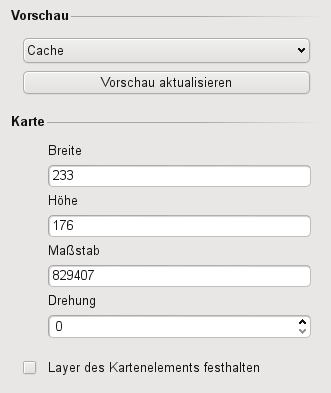
\includegraphics[clip=true, width=0.4\textwidth]{print_composer_map1}}
    \hspace{1cm}
  \subfloat[Panneau de l'emprise]{\label{subfig:map_dialog2}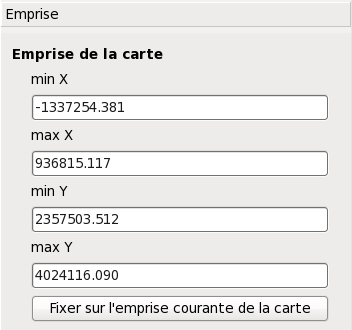
\includegraphics[clip=true, width=0.4\textwidth]{print_composer_map2}}
  \caption{Panneau de la carte et de l'emprise \nixcaption}\label{fig:mapdialog} 
\end{figure}

\minisec{Panneau de l'emprise}

%The \textbf{Extents} dialog of the map item tab provides following functionalities
%(see Figure \ref{fig:mapdialog}b)):
le panneau de l'\textbf{Emprise} de l'élément de la carte fournit les fonctionnalités suivantes (voir figure \ref{fig:mapdialog}b)):

%\begin{itemize}[label=--]
%\item The \textbf{Map extent} area allow to specify the map extend using Y
%and X min/max values or clicking the \button{Set to map canvas extend} button.
%\end{itemize}
\begin{itemize}[label=--]
\item La zone \textbf{Emprise de la carte} permet de spécifier l'étendue de la représentation cartographique en utilisant les valeurs X/Y minimales et maximales ou en cliquant sur le bouton  \button{Fixer sur l'emprise courante de la carte}.
\end{itemize}

%If you change the view on the QGIS map canvas by zooming or panning or
%changing vector or raster properties, you can update the print composer view
%selecting the map element in the print composer and clicking the
%\button{Update preview} button in the map \tab{Item} tab (see
%Figure~\ref{fig:mapdialog}a)).
Si vous changez de vue sur le canevas de la carte de QGIS en zoomant, en vous déplaçant ou en changeant les paramètres du vecteur ou raster, vous pouvez mettre à jour l'aperçu du composeur en sélectionnant l'élément de la carte et en cliquant le bouton \button{Mise à jour de l'aperçu} dans le panneau  \tab{objet} (voir figure~\ref{fig:mapdialog}a)).

%\subsection{Map item tab - Grid and General options dialog}
\subsection{Map item tab - Grid and General options dialog}

\begin{figure}[ht]
\centering
   \subfloat[Grille]{\label{subfig:map_dialog3}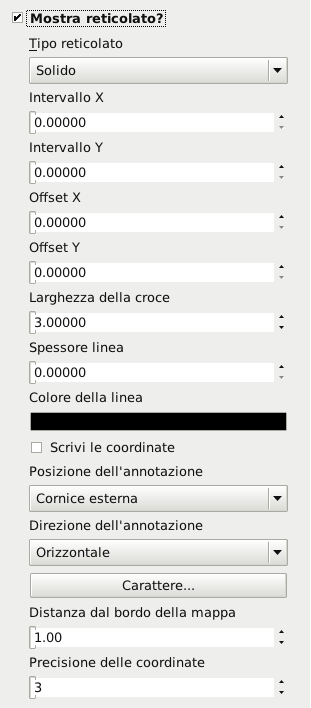
\includegraphics[clip=true, width=0.4\textwidth]{print_composer_map3}}
   \hspace{1cm}
   \subfloat[Options générales]{\label{subfig:map_dialog4}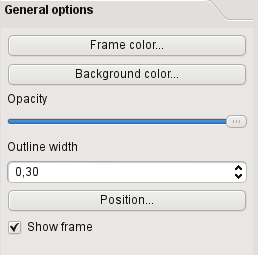
\includegraphics[clip=true, width=0.4\textwidth]{print_composer_attribute2}}
%   \caption{Print Composer map item tab - Grid and General options dialog \nixcaption}\label{fig:sec_map_dialog}
    \caption{Panneau de la carte - grille et options génériques \nixcaption}\label{fig:sec_map_dialog}
\end{figure}
\FloatBarrier
%\minisec{Grid dialog}
\minisec{Panneau de grille}

Le panneau de \textbf{Grille} de l'élément de carte dispose des fonctionnalités suivante (voir figure \ref{fig:sec_map_dialog}a)):

\begin{itemize}[label=--]
%\item The \checkbox{Show grid} checkbox allows to overlay a grid to the map
%element. As grid type you can specify to use solid line or cross. Furthermore
%you can define an interval in X and Y direction, an X and Y offset, and the
%width used for cross or line grid type.
\item La case \checkbox{Afficher le graticule} permet de superposer une grille sur l'élément de la carte. Vous pouvez choisir de la représenter sous forme de lignes continues ou de croix, choisir l'intervalle d'espacement dans les directions X et Y et les propriétés graphiques (couleur, épaisseur, etc.)
%\item The \checkbox{Draw annotation} checkbox allows to add coordinates to
%the map frame. The annotation can be drawn inside or outside the map frame.
%As annotatiion direction can be defined horizontal, vertical, horizontal and
%vertical or boundary direction. And finally you can define the grid color,
%the annotation font, the annotation distance from the map frame and the
%precision of the drawn coordinates.  
\item La case \checkbox{Dessiner une annotation} permet l'affichage des coordonnées sur le contour de la carte. Les annotations peuvent être placées à l'intérieur ou à l'extérieur tandis que leur direction peut être horizontale, verticale, horizontale et verticale ou dans le sens de la limite. Vous pouvez aussi choisir le type de police, la distance séparant l'annotation du cadre et la précision des coordonnées. 
\end{itemize}

%\minisec{General options dialog}
\minisec{Panneau des options globales}

%The \textbf{General options} dialog of the map item tab provides following
%functionalities (see Figure \ref{fig:sec_map_dialog}b)):
Le panneau \textbf{options globales} de l'élément de carte dispose des fonctionnalités suivante (voir figure \ref{fig:sec_map_dialog}b)):

%\begin{itemize}[label=--]
%\item Here you can define color and outline width for the element frame, set
%a background color and opacity for the map canvas. The \button{Position}
%button opens the \dialog{Set items position} dialog and allows to set the map
%canvas position using reference points or coordinates. Furthermore you can
%select or unselect to display the element frame with the \checkbox{Show
%frame} checkbox. 
%\end{itemize}
\begin{itemize}[label=--]
\item Vous pouvez définir ici la couleur et l'épaisseur du cadre de l'élément, choisir une couleur pour le fond et le niveau d'opacité de la carte. Le bouton \button{Position} ouvre la fenêtre \dialog{Définir la position de l'objet} qui permet de configurer la position du canevas de la carte en utilisant des points de référence ou des coordonnées. De plus, vous pouvez sélectionner ou désélectionner l'affichage du cadre de l'objet avec la case \checkbox{Afficher le cadre}. 
\end{itemize}

% \subsection{Adding other elements to the Print Composer}
\subsection{Ajouter d'autres éléments au Composeur d'Impression}

%Besides adding a current QGIS map canvas to the Print Composer, it is also possible 
%to add, position, move and customize legend, scalebar, images and label elements.
Au-delà de l'ajout d'un cadre de la carte actuelle de QGIS au composeur de carte, il est également possible d'ajouter, déplacer et personnaliser les
éléments légendes, échelles graphiques, images et étiquettes.

%\subsection{Label item tab - Label and General options dialog}
\subsection{Fenêtre des étiquettes}

%To add a label, click the \toolbtntwo{mActionLabel}{Add label} icon, place
%the element with the left mouse button on the print composer canvas and
%position and customize their appearance in the label item tab. 
Pour ajouter une étiquette, , cliquez sur l'icône \toolbtntwo{mActionLabel}{Ajouter une étiquette} et placez l'élément sur le canevas de la carte avec le bouton gauche de votre souris. Vous pouvez modifier la position et l'apparence avec le panneau de propriétés d'objets après avoir sélectionné l'élément.

\begin{figure}[ht]
\centering
   \subfloat[Options d'étiquetage]{\label{subfig:labeloptions1}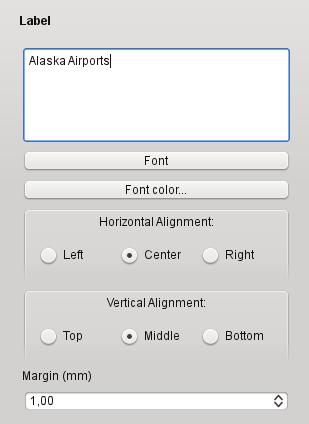
\includegraphics[clip=true, width=0.4\textwidth]{print_composer_label1}}
   \hspace{1cm}
   \subfloat[Options globales]{\label{subfig:labeloptions2}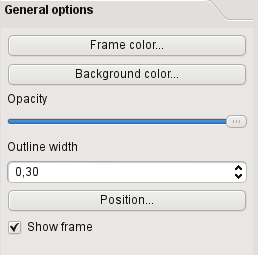
\includegraphics[clip=true, width=0.4\textwidth]{print_composer_attribute2}}
   \caption{Panneau des étiquettes de la composition - Options d'étiquetage et options globales \nixcaption}\label{fig:label_option}
\end{figure}

%\minisec{Label dialog}
\minisec{Panneau des étiquettes}

Le panneau \textbf{Étiquette} dispose des fonctionnalités suivantes (voir figure \ref{fig:label_option}a)):

\begin{itemize}[label=--]
%\item The \textbf{Label} dialog offers to add text labels to the composer
% canvas. You can define the horizontal and vertical alignment, select font 
% and fontcolor for the text and it is possible to define a text margin im mm.
\item Cette fenêtre permet d'ajouter des éléments textuel à la carte composée. Vous pouvez sélectionner l'alignement horizontal et vertical, la police et sa couleur ainsi que définir la marge en mm.
\end{itemize}

%\minisec{General options dialog}
\minisec{Panneau des options globales}

Le panneau \textbf{Options globales} dispose des fonctionnalités suivantes (voir figure \ref{fig:label_option}b)):

\begin{itemize}[label=--]
%\item Here you can define color and outline width for the element frame, set
%a background color and opacity for the label. The \button{Position}
%button opens the \dialog{Set items position} dialog and allows to set the map
%canvas position using reference points or coordinates. Furthermore you can
%select or unselect to display the element frame with the \checkbox{Show
%frame} checkbox.
\item Vous pouvez ici choisir la couleur et le contour du cadre de l'élément, mettre une couleur de fond et gérer l'opacité de l'étiquette. Le bouton \button{Position} ouvre la fenêtre \dialog{Définir la position de l'objet} qui permet de configurer la position du canevas de la carte en utilisant des points de référence ou des coordonnées. De plus, vous pouvez sélectionner ou désélectionner l'affichage du cadre de l'objet avec la case \checkbox{Afficher le cadre}.
\end{itemize}

%\subsection{Image item tab - Picture options and General options dialog}
\subsection{ Fenêtre des options d'images}

%To add an image, click the \toolbtntwo{mActionSaveMapAsImage}{Add image}
%icon, place the element with the left mouse button on the print composer
%canvas and position and customize their appearance in the image item tab.
Pour ajouter une image, cliquez sur l'icône \toolbtntwo{mActionSaveMapAsImage}{Ajouter une image} et placez l'élément sur le canevas de la carte avec le bouton gauche de votre souris. Vous pouvez modifier la position et l'apparence avec le panneau de propriétés d'objets après avoir sélectionné l'élément.

%\begin{figure}[ht]
%\centering
%   \subfloat[Picture options dialog]{\label{subfig:print_composer_image1}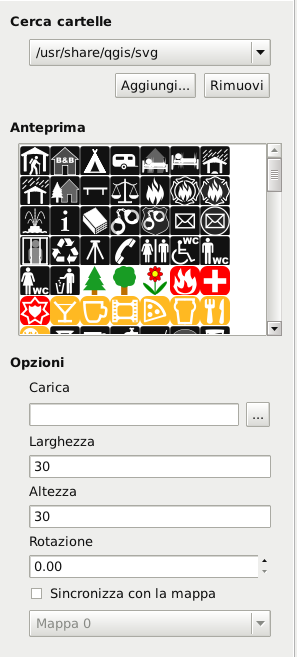
\includegraphics[clip=true, width=0.30\textwidth]{print_composer_image1}}
%     \hspace{1cm}
%   \subfloat[General options dialog]{\label{subfig:print_composer_image2}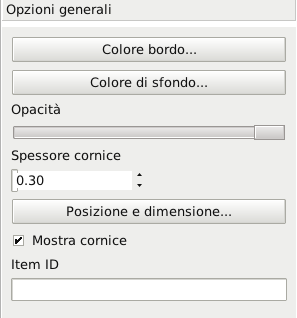
\includegraphics[clip=true, width=0.4\textwidth]{print_composer_image2}}
%   \caption{Print composer image item tab - Picture options and General options \nixcaption}\label{fig:imageoptions}
%\end{figure}

\begin{figure}[ht]
\centering
   \subfloat[Fenêtre des options de l'image]{\label{subfig:print_composer_image1}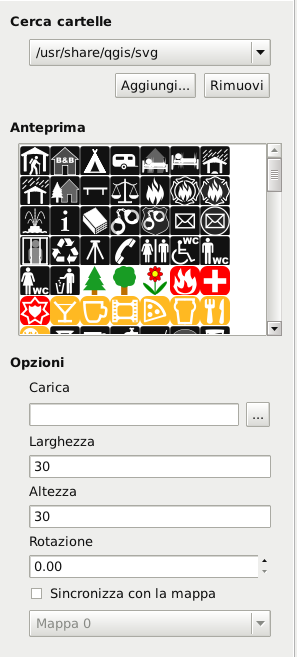
\includegraphics[clip=true, width=0.30\textwidth]{print_composer_image1}}
     \hspace{1cm}
   \subfloat[Fenêtre des options globales]{\label{subfig:print_composer_image2}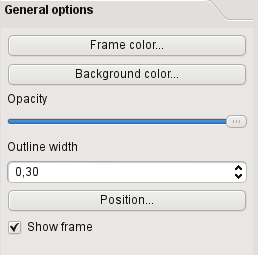
\includegraphics[clip=true, width=0.4\textwidth]{print_composer_attribute2}}
   \caption{Panneau d'image du composeur d'impression \nixcaption} \label{fig:imageoptions}
\end{figure}

%\minisec{Picture options dialog}
\minisec{Fenêtre des options de l'image}

%The \textbf{Picture options} dialog of the image item tab provides following
%functionalities (see Figure \ref{fig:imageoptions}a)):

La fenêtre \textbf{Options de l'image} dispose des fonctionnalités suivantes (voir figure \ref{fig:imageoptions}a)):

%\begin{itemize}[label=--]
%\item The \textbf{Search directories} area allows to add and remove
%directories with images in SVG format to the picture database. 
%\item The \textbf{Preview} field then shows all pictures stored in the
%selected directories.
%\item The \textbf{Options} area shows the current selected picture and allows
%to define width, height and clockwise rotation of the picture. It is also possible 
%to add a user specific SVG path. Activating the
%\checkbox{Sync from map} checkbox synchronizes the rotation of a picture in
%the qgis map canvas (i.e. a rotated north arrow) with the appropriate print
%composer image.
%\end{itemize}
\begin{itemize}[label=--]
\item La zone \textbf{Rechercher dans les répertoires} permet d'ajouter et d'effacer des répertoires contenant des images au format SVG à liste d'images à disposition.
\item Le champ \textbf{Aperçu} permet d'afficher une miniature pour chaque image stockée dans le répertoire sélectionné
\item La zone \textbf{Options} affiche l'image sélectionnée et permet de définir sa largeur, hauteur et rotation (dans le sens horaire). Il est possible de saisir un chemin vers une image spécifique. Le fait d'activer la case \checkbox{Synchroniser depuis la carte} permet à l'image de suivre la même rotation que la carte (P. ex. une flèche pointant ainsi toujours vers le Nord même si le contenu de la carte a été pivoté).
\end{itemize}

%\minisec{General options dialog}
\minisec{Fenêtre des options globales}

%The \textbf{General options} dialog of the image item tab provides following
%functionalities (see Figure \ref{fig:imageoptions}b)):
La fenêtre des \textbf{Options globales} dispose des fonctionnalités suivantes (voir figure \ref{fig:imageoptions}b)):

\begin{itemize}[label=--]
%\item Here you can define color and outline width for the element frame, set
%a background color and opacity for the picture. The \button{Position}
%button opens the \dialog{Set items position} dialog and allows to set the map
%canvas position using reference points or coordinates. Furthermore you can
%select or unselect to display the element frame with the \checkbox{Show
%frame} checkbox.
\item Vous pouvez ici choisir la couleur et le contour du cadre de l'image, mettre une couleur de fond et gérer son opacité. Le bouton \button{Position} ouvre la fenêtre \dialog{Définir la position de l'objet} qui permet de configurer la position du canevas de la carte en utilisant des points de référence ou des coordonnées. De plus, vous pouvez sélectionner ou désélectionner l'affichage du cadre de l'objet avec la case \checkbox{Afficher le cadre}.
\end{itemize}

%\subsection{Legend item tab - General, Legend items and Item option dialog }
\subsection{Fenêtre des options de la légende}

%To add a map legend, click the \toolbtntwo{mActionAddLegend}{Add new legend}
%icon, place the element with the left mouse button on the print composer
%canvas and position and customize their appearance in the legend item tab.
Pour ajouter une légende à la carte, cliquez sur l'icône \toolbtntwo{mActionAddLegend}{Ajouter une nouvelle légende}, placez l'élément sur le canevas de la carte avec le bouton gauche de votre souris. Vous pouvez modifier la position et l'apparence avec le panneau de propriétés d'objets après avoir sélectionné la légende.

\begin{figure}[h]
\centering
   \subfloat[Panneau général]{\label{subfig:print_composer_legend1}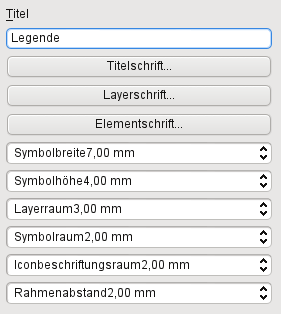
\includegraphics[clip=true, width=0.3\textwidth]{print_composer_legend1}}
   \hspace{1cm}
   \subfloat[Panneau des objets de la légende]{\label{subfig:print_composer_legend2}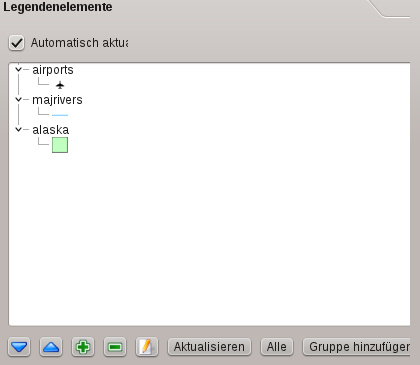
\includegraphics[clip=true, width=0.3\textwidth]{print_composer_legend2}}
   \hspace{1cm}
   \subfloat[Options des objets]{\label{subfig:print_composer_legend3}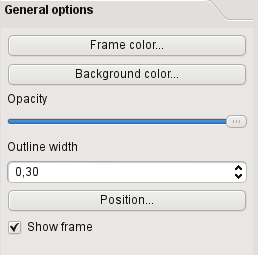
\includegraphics[clip=true, width=0.3\textwidth]{print_composer_attribute2}}
   \caption{Fenêtre des propriétés de la légende du composeur d'impression \nixcaption}\label{fig:legendoptions}
\end{figure}

%\minisec{General dialog}
\minisec{General dialog}

Le panneau \textbf{Général} dispose des fonctionnalités suivantes (voir figure \ref{fig:legendoptions}a)):

%\begin{itemize}[label=--]
%\item Here you can adapt the legend title. You can change the font of the
%legend title, layer and item name. You can change width and height of the
%legend symbol and you can add layer, symbol, icon label and box space.
%\end{itemize}
\begin{itemize}[label=--]
\item Vous pouvez ici modifier le titre de la légende et la police utilisée. Vous pouvez changer la hauteur et la largeur des symboles de la légende et ajouter des couches, des symboles, des icônes et des espaces.
\end{itemize}

%\minisec{Legend items dialog}
\minisec{Panneau des objets de la légende}

Le panneau \textbf{Objets de légende} dispose des fonctionnalités suivantes (voir figure \ref{fig:legendoptions}b)):

\begin{itemize}[label=--]
%\item The legend items window lists all legend items and allows to change
%item order, edit layer names, remove and restore items of the list. After
%changing the symbology in the QGIS main window you can click on \button{Update} to
%adapt the changes in the legend element of the print composer. The item oder 
%can be changed using the \button{Up} and \button{Down} buttons or with Drag and Drop 
%functionality. 
\item Cette fenêtre montre tous les objets inclus dans la légende et permet d'en changer l'ordre. Après avoir modifié la symbologie de QGIS dans la fenêtre principale de l'application, vous pouvez cliquer sur \button{Mise à jour} pour répercuter ces changements sur les objets de la légende du composeur d'impression. L'ordre des objets peut être altéré en utilisant les \button{monter} et \button{descendre} ou en faisant un glisser-déposer.
\end{itemize}

%\minisec{Item options dialog}
\minisec{Panneau des options des objets}

Le panneau \textbf{Options des objets} dispose des fonctionnalités suivantes (voir figure \ref{fig:legendoptions}c)):

%\begin{itemize}[label=--]
%\item Here you can define color and outline width for the element frame, set
%a background color and opacity for the legend. The \button{Position}
%button opens the \dialog{Set items position} dialog and allows to set the map
%canvas position using reference points or coordinates. Furthermore you can
%select or unselect to display the element frame with the \checkbox{Show
%frame} checkbox.
%\end{itemize}
\begin{itemize}[label=--]
\item Vous pouvez ici choisir la couleur et le contour du cadre de l'élément, mettre une couleur de fond et gérer son opacité. Le bouton \button{Position} ouvre la fenêtre \dialog{Définir la position de l'objet} qui permet de configurer la position du canevas de la carte en utilisant des points de référence ou des coordonnées. De plus, vous pouvez sélectionner ou désélectionner l'affichage du cadre de l'objet avec la case \checkbox{Afficher le cadre}.
\end{itemize}

%\subsection{Scalebar item tab - Scalebar and General options dialog}
\subsection{Fenêtre des options de la barre d'échelle}

%To add a scalebar, click the \toolbtntwo{mActionScaleBar}{Add new scalebar}
%icon, place the element with the left mouse button on the print composer
%canvas and position and customize their appearance in the scalebar item tab.
Pour ajouter une barre d'échelle, cliquez sur l'icône \toolbtntwo{mActionScaleBar}{Ajouter une nouvelle échelle graphique}, placez l'élément sur le canevas de la carte avec le bouton gauche de votre souris. Vous pouvez modifier la position et son apparence avec le panneau de propriétés d'objets après avoir sélectionné l'élément.

\begin{figure}[ht]
\centering
\subfloat[Panneau des options de la barre]{\label{subfig:scalebaroptions1}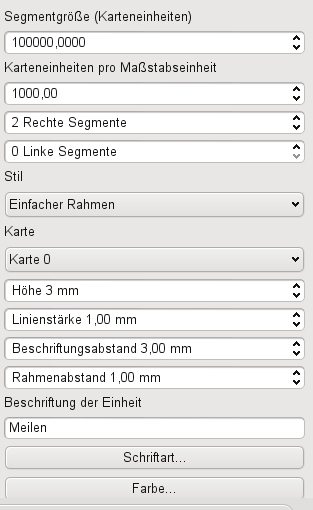
\includegraphics[clip=true, width=0.35\textwidth]{print_composer_scalebar1}}
\hspace{1cm}
\subfloat[Panneau des options globales]{\label{subfig:scalebaroptions2}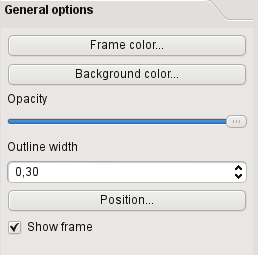
\includegraphics[clip=true, width=0.4\textwidth]{print_composer_attribute2}}
\caption{Panneaux de la barre d'échelle graphique du composeur d'impression \nixcaption}\label{fig:scalebaroptions}
\end{figure}

%\minisec{Scalebar dialog}
\minisec{Panneau de l'échelle graphique}

La \textbf{Barre d'échelle} dispose des fonctionnalités suivantes (voir figure \ref{fig:scalebaroptions}a)):

\begin{itemize}[label=--]
%\item The scalebar dialog allows to define the segment size of the scalebar
%in map units, the map units used per bar units, and how many left and right
%segments units from 0 should be used.
%\item You can define the scalebar style, available is single and double box,
%line ticks middle, up and down and a numeric style.
%\item Furthermore you can define height, line width, label and box space of
%the scale bar. Add a unit label and define the scalebar font and color.
\item Ce panneau permet de définir la taille de segment de l'échelle en unités de la carte, les unités de la carte par unité de la barre et combien de segments doivent apparaître à droite et à gauche du 0. 
\item Vous pouvez changer le style de la barre d'échelle, disponible avec un ou 2 niveaux de segments, plate avec des repères ajustables ou simplement numérique (1:500). 
\item Il est également possible de la hauteur, l'épaisseur des traits, la police des unités, les différents espaces ainsi que l'étiquette des unités.
\end{itemize}

%\minisec{General options dialog}
\minisec{Options globales}

%The \textbf{General options} dialog of the scalebar item tab provides following
%features (see Figure \ref{fig:scalebaroptions}b)):
Le panneau \textbf{Options globales} dispose des fonctionnalités suivantes (voir figure  \ref{fig:scalebaroptions}b)):

%\begin{itemize}[label=--]
%\item Here you can define color and outline width for the element frame, set
%a background color and opacity for the scalebar. The \button{Position}
%button opens the \dialog{Set items position} dialog and allows to set the map
%canvas position using reference points or coordinates. Furthermore you can
%select or unselect to display the element frame with the \checkbox{Show
%frame} checkbox.
%\end{itemize}
\begin{itemize}[label=--]
\item Vous pouvez ici choisir la couleur et le contour du cadre de l'élément, mettre une couleur de fond et gérer son opacité. Le bouton \button{Position} ouvre la fenêtre \dialog{Définir la position de l'objet} qui permet de configurer la position du canevas de la carte en utilisant des points de référence ou des coordonnées. De plus, vous pouvez sélectionner ou désélectionner l'affichage du cadre de l'objet avec la case \checkbox{Afficher le cadre}.
\end{itemize}

%\section{Navigation tools}
\section{Outils de navigation}

%For map navigation the print composer provides 4 general tools:
Pour vous déplacer sur la carte, le composeur d'impression propose 4 outils :

\begin{itemize}[label=--]
\item \toolbtntwo{mActionZoomIn}{Zoom +},
\item \toolbtntwo{mActionZoomOut}{Zoom -},
\item \toolbtntwo{mActionZoomFullExtent}{Zoom sur l'étendue totale} et
\item \toolbtntwo{mActionDraw}{Rafraîchir la vue} pour actualiser l'affichage si nécessaire
\end{itemize}

\section{Ajouter des formes basiques et des flèches}

%It is possible to add basic shapes (Ellipse, Rectangle, Triangle) and arrows
%to the print composer canvas. 
Il est possible d'ajouter des formes simples (Ellipse, Rectangle, Triangle) et des flèches à la composition.

\begin{figure}[ht]
\centering
\subfloat[Panneau des formes]{\label{subfig:shapedialog}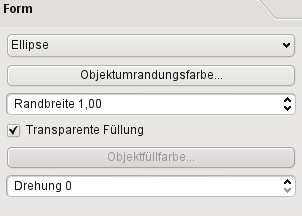
\includegraphics[clip=true, width=0.35\textwidth]{print_composer_shape}}
\hspace{1cm}
\subfloat[Panneau des flèches]{\label{subfig:arrowdialog}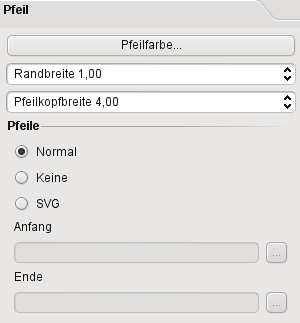
\includegraphics[clip=true, width=0.35\textwidth]{print_composer_arrow}}
\caption{Panneaux des formes basiques et flèches \nixcaption}\label{fig:shapearrow}
\end{figure}

%\begin{itemize}[label=--]
%\item The \textbf{Shape} dialog allows to draw an ellipse, rectangle, or
%triangle in the print composer canvas. You can define its outline and fill
%color, the outline width and a clockwise rotation.
%\item The \textbf{Arrow} dialog allows to draw an arrow in the print composer
%canvas. You can define color, outline and arrow width and it is possible to
%use a default marker and no marker and a SVG marker. For the SVG marker you
%can additionally add a SVG start and end marker from a directory on your
%computer.
%\end{itemize}
\begin{itemize}[label=--]
\item Le panneau \textbf{Forme} permet de dessiner une ellipse, un rectangle, ou un triangle. Vous pouvez modifier le contours, la couleur de remplissage et la rotation (dans le sens horaire).
\item Le panneau  \textbf{Flèche} permet de dssiner une flèche sur la carte, vous permettant d'attirer l'attention sur une partie spécifique de votre composition. Vous pouvez changer la couleur, le contour et la taille de la flèche. Il est possible d'utiliser un marqueur par défaut pour la pointe, aucun marqueur ou un marqueur SVG. Dans le cas du marqueur SVG, vous pouvez en placer un à la fin du trait et un autre au début.
\end{itemize}

\section{Ajouter une table attributaire}

%It is possible to add parts of a vector attribute table to the print composer canvas.
Vous pouvez ajouter une table attributaire d'une couche vectorielle sur la composition de la carte.

\begin{figure}[ht]
\centering
\subfloat[Panneau de la table]{\label{subfig:tabledialog1}\includegraphics[clip=true, width=0.38\textwidth]{print_composer_attribute1}}
\hspace{1cm}
\subfloat[Options globales]{\label{subfig:tabledialog2}\includegraphics[clip=true, width=0.38\textwidth]{print_composer_attribute2}}
\caption{Panneau de table attributaire du composeur de carte \nixcaption}\label{fig:attrcomp}
\end{figure}

\minisec{Panneau de table}

%The \textbf{Table} dialog of the attribute table item tab provides following
%functionalities (see Figure \ref{fig:attrcomp}a)):
Le panneau \textbf{Table} dispose des fonctionnalités suivantes (voir figure  \ref{fig:attrcomp}a)):

%\begin{itemize}[label=--]
%\item The \textbf{Table} dialog allows to select the vector layer and columns of 
% the attribute table. Attribute columns can be sorted and you can define to show 
% its values ascending or descending. 
% \item You can define the maximum number of rows to be displayed
%and if attributes are only shown for visible features of the current composer 
% canvas. 
% \item Additionally you can define the grid characteristics of the table and
%the header and content font. 
%\end{itemize}
\begin{itemize}[label=--]
\item Le panneau \textbf{Table} permet de sélectionner une couche vectorielle et d'en afficher les colonnes avec la carte. Les colonnes peuvent être triées dans un ordre descendant ou ascendant.
\item Vous pouvez limiter le nombre d'enregistrements affichés ou limiter aux entités affichés dans votre composition.
\item Vous pouvez modifier les caractétristiques de grille du tableau ainsi que l'en-tête et la police employée.
\end{itemize}

%\minisec{General options dialog}
\minisec{Options globales}

%The \textbf{General options} dialog of the attribute table item tab 
%provides following functionalities (see Figure \ref{fig:attrcomp}b)):
Le panneau \textbf{Options globales} dispose des fonctionnalités suivantes (voir figure  \ref{fig:attrcomp}b)):

%\begin{itemize}[label=--]
%\item Here you can define color and outline width for the element frame, set
%a background color and opacity for the table. The \button{Position}
%button opens the \dialog{Set items position} dialog and allows to set the map
%canvas position using reference points or coordinates. Furthermore you can
%select or unselect to display the element frame with the \checkbox{Show
%frame} checkbox.
%\end{itemize}
\begin{itemize}[label=--]
\item Vous pouvez ici choisir la couleur et le contour du cadre de l'élément, mettre une couleur de fond et gérer son opacité. Le bouton \button{Position} ouvre la fenêtre \dialog{Définir la position de l'objet} qui permet de configurer la position du canevas de la carte en utilisant des points de référence ou des coordonnées. De plus, vous pouvez sélectionner ou désélectionner l'affichage du cadre de l'objet avec la case \checkbox{Afficher le cadre}.
\end{itemize}

%\subsection{Raise, lower and align elements}
\subsection{Monter, descendre et aligner des éléments}

%Raise or lower functionalities for elements are inside the
%\toolbtntwo{mActionRaiseItems}{Raise selected items} pulldown menu. Choose an
%element on the print composer canvas and select the matching functionality to
%raise or lower the selected element compared to the other elements (see
%table~\ref{tab:printcomposer_tools}). 
Les fonctionnalités pour relever ou descendre des éléments sont présentes dans le menu déourlant \toolbtntwo{mActionRaiseItems}{Relever les objets sélectionnés}. Prenez un élément dans le composeur de carte et sélectionnez la fonction correspondante pour le relever ou le descendre par rapport aux autres éléments (voir table~\ref{tab:printcomposer_tools}).

%There are several alignment functionalities available within the
%\toolbtntwo{mActionAlignLeft}{Align selected items} pulldown menu (see
%table~\ref{tab:printcomposer_tools}). To use an alignment functionality , you
%first select some elements and then click on the matching alignment icon. All
%selected will then be aligned within to their common bounding box.
Il y a plusieurs fonctionnalités d'alignements disponibles dans le menu déroulant\\ \toolbtntwo{mActionAlignLeft}{Aligner les objets sélectionnés} (voir table~\ref{tab:printcomposer_tools}). Pour utiliser une fonction, vous devez d'abord sélectionner plusieurs éléments et ensuite cliquer sur l'icône d'alignement désiré. Toute la sélection sera alignée dans le cadre de leurs limites respectives

% \subsection{Creating Output}
\subsection{Création de carte}

% Figure \ref{fig:print_composer_complete} shows the print composer with an
% example print layout including each type of map element described in the
% sections above.
La figure \ref{fig:print_composer_complete} montre le composeur de carte avec
un exemple de mise en page incluant chaque type d'élément de la carte décrit
dans la section au-dessus.

\begin{figure}[ht]
   \begin{center}
%    \caption{Print Composer with map view, legend, scalebar, and text added
\smallskip
   \includegraphics[clip=true, width=\textwidth]{print_composer_complete}
   \caption{Composeur comportant une vue de la carte, une légende, une échelle graphique et du texte ajouté \nixcaption}
   \label{fig:print_composer_complete}
\end{center}
\end{figure}

% The print composer allows you to create several output formats and it is
% possible to define the resolution (print quality) and paper size:
Le composeur de carte vous permet de choisir plusieurs formats de sortie et il est possible de définir la résolution (qualité d'impression) et la taille du papier :

\begin{itemize}[label=--]
% \item The \toolbtntwo{mActionFilePrint}{Print} icon allows to print the
% layout to a connected printer or as PDF or Postscript file depending on
% installed printer drivers.
\item L'icône \toolbtntwo{mActionFilePrint}{Imprimer}  permet d'imprimer la mise en page à une imprimante ou dans un fichier Postscript en fonction des pilotes d'imprimante installés.
%\item The \toolbtntwo{mActionSaveAsPDF}{Export as PDF} saves the defined
%print composer canvas directly as a PDF.
\item The \toolbtntwo{mActionSaveAsPDF}{Exporter au format PDF} enregistre le contenu du composeur directement dans un fichier PDF.
% \item The \toolbtntwo{mActionExportMapServer}{Export as image} icon exports
% the composer canvas in several image formats such as PNG, BPM, TIF, JPG, \dots
\item L'icône \toolbtntwo{mActionExportMapServer}{Exporter dans une image} exporte le cadre du composeur dans plusieurs formats d'image tels que PNG, BPM,TIF, JPG, \dots

% \item The \toolbtntwo{mActionSaveAsSVG}{Export as SVG} icon saves the print 
% composer canvas as a SVG (Scalable Vector Graphic). \textbf{Note:} Currently
% the SVG output is very basic. This is not a QGIS problem, but a problem of the
% underlaying Qt library. This will hopefully be sorted out in future versions.
\item L'icône \toolbtntwo{mActionSaveAsSVG}{Exporter au format SVG} sauve le cadre du composeur de carte en SVG (Scalable Vector Graphic). \textbf{Note :} Actuellement la sortie SVG est très basique. Ce n'est pas un problème de QGIS mais un problème de la bibliothèque Qt sous-jacente. Cela sera
probablement corrigé dans une prochaine version. \end{itemize}

%\subsection{Saving and loading a print composer layout}
\subsection{Enregistrer et charger une mise en page d'impression}

%With the \toolbtntwo{mActionFileSaveAs}{Save as template} and
%\toolbtntwo{mActionFolder}{Load from template} icons you can save the current
%state of a print composer session as a  *.qpt template and load the template
%again in another session.
Avec les icônes \toolbtntwo{mActionFileSaveAs}{Sauvegarder en tant que modèle} et \toolbtntwo{mActionFolder}{Charger depuis un modèle}, vous pouvez enregistrer l'état actuel d'une session du composeur dans un modèle *.qpt et le charger dans une autre session.

%\section{Saving and loading a print composer layout}
\section{Enregistrer et charger une composition de carte}

%With the \toolbtntwo{mActionFileSaveAs}{Save as template} and
%\toolbtntwo{mActionFolder}{Load from template} icons you can save the current
%state of a print composer session as a  *.qpt template and load the template
%again in another session.
Avec les icônes \toolbtntwo{mActionFileSaveAs}{Sauvegarder le modèle} and \toolbtntwo{mActionFolder}{Charger un modèle}, vous pouvez enregistrer l'état actuel de votre session de composition dans un fichier *.qpt que vous pourrez recharger dans une session suivante.

%The  \toolbtntwo{mActionComposerManager}{Composer Manager} button in the
%toolbar and in \mainmenuopt{File} >
%\dropmenuopttwo{mActionComposerManager}{Composer Manager} allows to manage
%add new composer template or to manage already existing templates. 
Le bouton \toolbtntwo{mActionComposerManager}{Gestionnaire de composition} qui se situe dans la barre d'outils et dans le menu \mainmenuopt{Fichier} > \dropmenuopttwo{mActionComposerManager}{Gestionnaire de composition} permet de gérer l'ajout de nouveau modèle à votre projet (p. ex. en chargeant un modèle externe) ou de gérer les modèles existants.

\begin{figure}[h]
   \centering
   \includegraphics[clip=true, width=8cm]{print_composer_manager}   
   \caption{Gestionnaire de composition \nixcaption}
   \label{fig:print_composer_manager}
\end{figure}

\FloatBarrier
